\section{El agua}

	El planeta Tierra es conocido como planeta azul debido a que el \percent{70} de su superficie está cubierta de agua, a pesar de ello, solamente el \percent{0.025} de ella es potable. El \percent{97.5} corresponde a al agua salada de mares y océanos; del \percent{2.5} restante \percent{80} está congelada en casquetes polares, glaciares o se encuentra como humedad del suelo y no se considera accesible. El resto se encuentra en el subsuelo, pozos, acuíferos, cuencas hidrográficas, ríos y arroyos \cite{el-dessouky_chapter_2002}.
	
	\subsection{Clasificaciones del agua}
	
		El agua puede clasificarse de distintas formas, entre las cuales se puede considerar el \acrfull{tsd}. En la~\cref{table:clasificacion-agua-tds} se puede observar la clasificación propuesta por la \acrfull{wqa}.
		
		\begin{longtblr}[
			caption = {Clasificación del agua con respecto al \acrshort{tsd} según \acrshort{wqa}},
			label = {table:clasificacion-agua-tds},
			remark{Referencia} = {Datos obtenidos del glosario en línea de la \acrshort{wqa} \cite{water_quality_association_glossary_nodate}}
		]{
			colspec = {*{2}{X[c]}},
			width=0.7\textwidth,
			hlines,
			vlines,
			row{odd} = {bg=tablerowblue},
			row{1} = {
				bg = tabletitleblue,
				fg=white,
				font =  \large\bfseries
			},
			rowhead = 1,
			rows={m},
		}
			{Denominación} & TSD (\unit[per-mode = symbol]{\mg\per\litre})\\ 
			% Table body%
			Agua fresca & menor a \num{1000}\\
			Agua salobre & entre \num{1000} y \num{5000}\\
			Agua altamente salobre & entre \num{5000} y \num{15000}\\
			Agua salina & entre \num{15000} y \num{30000}\\
			Agua de mar & entre \num{30000} y \num{40000}\\
			Salmuera & entre \num{40000} y \num{300000}+\\
		\end{longtblr}
		
		Otra forma de clasificar el agua es de acuerdo a su forma final de uso y la salinidad que presenta. En la~\cref{table:clasificacion-agua-dessouky} se describe la relación entre el grado de salinidad y su uso en sectores de la población.
		
		\begin{talltblr}[
			caption = {Clasificación del agua propuesta por \cite{el-dessouky_chapter_2002} de acuerdo a su uso},
			label = {table:clasificacion-agua-dessouky}
		]{
			colspec = {X[c] X[0.75, c] X[c]},
			width=\textwidth,
			hlines,
			vlines,
			row{odd} = {bg=tablerowblue},
			row{1} = {
				bg = tabletitleblue,
				fg=white,
				font =  \large\bfseries
			},
			rowhead = 1,
			rows={m},
			cell{3}{3} = {r=2}{valign = m}
		}
			{Categoría} & Salinidad (ppm) & Fuentes\\ 
			% Table body%
			Industrias como la farmacéutica, eléctrica o de evaporación en calderas
				& menor a \num{5}
				& Ríos de muy baja salinidad o plantas desalinizadoras\\
			Agua potable
				& menor a \num{150}
				& Ríos, Lagos, plantas desalinizadoras\\
			Agua para uso doméstrico 
				& entre \num{150} y \num{1000}
				&~\\
			Riego y refrigeración industrial
				& entre \num{1000} y \num{3000}
				& Agua salobre y agua de mar\\		
		\end{talltblr}
	
	\subsection{Composición del agua de mar}
	
		El agua de mar es una mezcla compleja de aproximadamente \percent{96.5} de agua y \percent{2.5} de sales y en menor cantidad otras sustancias incluyendo sustancias orgánicas e inorgánicas disueltas \cite{alyn_c_duxbury_seawater_2023}. Al analizarla se identifican seis iones predominantes los cuales pueden ser observados en la~\cref{table:ionic-composition-of-seawater} junto a otros iones en menor cantidad.
			
			\begin{longtblr}[
				caption = {Principales iones constituyentes del agua de mar},
				label = {table:ionic-composition-of-seawater},
				remark{Nota} = {Concentración de salinidad igual a \num{34.7}},
				remark{Referencia} = {Tabla traducida de \cite{alyn_c_duxbury_seawater_2023}}
			]{
				colspec = {*{4}{X[c]}},
				width=\textwidth,
				hlines,
				vlines,
				row{odd} = {bg=tablerowblue},
				row{1} = {
					bg = tabletitleblue,
					fg=white,
					font =  \large\bfseries
				},
				rowhead = 1,
				rows={m}
			}
				Constituyente iónico
					& Compuesto químico
					& \unit{\gram\per\kg\ de\ agua}
					& \unit{\mole\per\kg\ de\ agua}\\
				Cloruro
					& \ch{Cl\mch}
					& 19.162
					& 0.5405\\
				Sodio
					& \ch{Na\pch}
					& 10.679
					& 0.4645\\
				Magnesio
					& \ch{Mg\pch[2]}
					& 1.278
					& 0.0526\\
				Sulfato
					& \ch{(SO4)\mch[2]}
					& 2.680
					& 0.0279\\
				Calcio
					& \ch{Ca\pch[2]}
					& 0.4096
					& 0.01022\\
				Potasio
					& \ch{K\pch}
					& 0.3956
					& 0.01011\\
				Ácido carbónico
					& \ch{(CO3)\mch[2]}
					& 0.0276
					& 0.0023\\
				Bromuro
					& \ch{Br\mch}
					& 0.0663
					& 0.00083\\
				Boro
					& \ch{B}
					& 0.0044
					& 0.00041\\
				Estroncio
					& \ch{Sr\pch[2]}
					& 0.0079
					& 0.00009\\
				Fluoruro
					& \ch{F\mch}
					& 0.0013
					& 0.00007
			\end{longtblr}
			
			Se ha observado que los constituyentes descritos en la~\cref{table:ionic-composition-of-seawater} son constantes ya que el tiempo que se necesita para una mezcla uniforme es muy corto en comparación al tiempo requerido para remover o quitar por completo uno de los constituyentes, aunque estos datos pueden cambiar ligeramente por la evaporación o la precipitación por ejemplo.
			
			
	\subsection{El efecto de la salinidad sobre el agua}
			
		Obianyo \cite{obianyo_effect_2019} realizó un experimento con diferentes sales y cantidades para observar cómo afecta la salinidad la capacidad de evaporación del agua; su estudio nos indica que hay una relación clara entre el aumento de la salinidad y la reducción de la evaporación. Los coeficientes de retardo se pueden observar en la~\cref{table:retardo-evaporacion-sal}.
		
		En el \cref{ch:seawater-properties} podemos observar la variación de las propiedades del agua de mar conforme a la salinidad a una atmósfera de presión, en el que se puede corroborar la relación de la salinidad y diversas propiedades vinculadas a la evaporación.
		
		\begin{minipage}[c]{0.5\linewidth}
			\begin{talltblr}[
				caption = {Factores de retardo en la evaporación de agua con diferentes sales},
				label = {table:retardo-evaporacion-sal}
			]{
				colspec = {c c},
				hlines,
				vlines,
				row{odd} = {bg=tablerowblue},
				row{1} = {
					bg = tabletitleblue,
					fg=white,
					font =  \large\bfseries
				},
				rowhead = 1,
				rows={m},
			}
				
				{Sal} & Factor de retraso\\ 
				% Table body%
				Sulfato de magnesio & \num{0.800}\\
				Hidróxido de sodio & \num{0.490}\\
				Cloruro de sodio & \num{0.712}\\
				Cloruro de amonio & \num{0.820}\\
				Nitrato de potasio & \num{0.822}\\
			\end{talltblr}
		\end{minipage}
		\hfill
		\begin{minipage}[c]{0.45\linewidth}
			\begin{figure}[H]
				\centering
				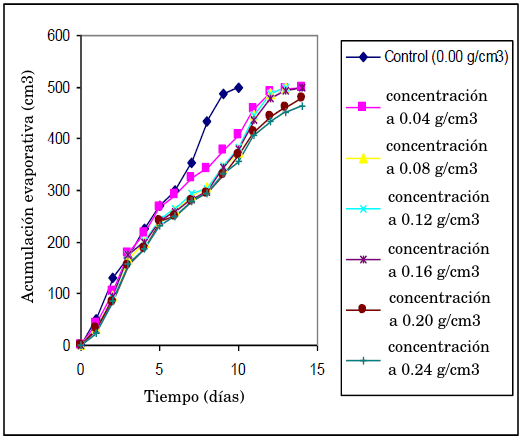
\includegraphics[width=\linewidth, keepaspectratio]{Marco-teórico/nacl-evaporation.png}
				\caption{Relación entre la evaporación acumulada y el tiempo para la solución NaCl}
				\floatfoot{Figura traducida de \cite{obianyo_effect_2019}}
				\label{fig:relacion-evaporación-sal}
			\end{figure}
		\end{minipage}
		
	\subsection{Propiedades coligativas del agua}
			
		El agua es un solvente por excelencia, por ello, en un proceso de desalinización se deben tomar en cuenta \gls{propiedades_coligativas} de las soluciones:
		
		\begin{itemize}[columns=2]
			\item Reducción relativa de la presión de vapor
			\item Elevación del punto de ebullición
			\item Depresión en el punto de congelación
			\item Presión osmótica
		\end{itemize}
		
		\subsubsection{Elevación del punto de ebullición y disminución de la presión de vapor}
			
			La elevación del punto de ebullición es proporcional a la molaridad de la solución. Este fenómeno se puede explicar a través de la presión de vapor.
			
			\begin{displayquote}
				La presión de vapor del líquido puro refleja la tendencia de la solución hacia una mayor entropía, que se puede lograr si el líquido se vaporiza para formar un gas. Cuando un soluto está presente, hay una contribución adicional a la entropía del líquido, incluso en una solución ideal. Debido a que la entropía del líquido ya es más alta que la del líquido puro, hay una tendencia más débil a formar el gas (\cref{fig:coligativas-pv}). El efecto del soluto aparece como una presión de vapor baja, y por lo tanto un punto de ebullición más alto. Del mismo modo, la aleatoriedad molecular mejorada de la solución se opone a la tendencia a congelarse. En consecuencia, se debe mantener una temperatura más baja antes de alcanzar el equilibrio entre el sólido y la solución. Por lo tanto, el punto de congelación se reduce. \cite{atkins_physical_2010}.
			\end{displayquote}
			\begin{figure}[H]
				\centering
				\begin{subfigure}[t]{0.45\linewidth}
					\centering
					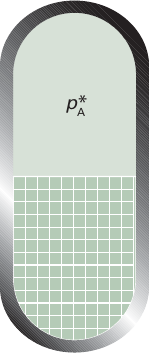
\includegraphics[width=\linewidth, height=50mm, keepaspectratio]{
						Marco-teórico/atkins-a.png
					}
					\caption{Se imagina a un solvente líquido como una estructura de cuadros}
				\end{subfigure}
				\hfill
				\begin{subfigure}[t]{0.45\linewidth}
					\centering
					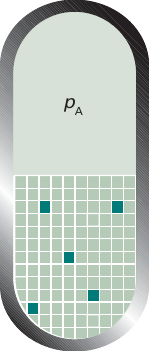
\includegraphics[width=\linewidth, height=50mm, keepaspectratio]{
						Marco-teórico/atkins-b.png
					}
					\caption{Cuando hay presencia de un soluto (cuadros oscuros), la entalpía es más grande a comparación de un líquido puro y por ello hay una decreciente tendencia a adquirir el desorden característico de un vapor}
				\end{subfigure}
				
				\caption{La presión de vapor de un líquido puro representa el balance entre el aumento de entalpía debido a la vaporización y la disminución de entalpía en su entorno.}
				\floatfoot{Figuras obtenidas de \cite{atkins_physical_2010}}
				\label{fig:coligativas-pv}
			\end{figure}